\subsection{内存管理}

\subsubsection{概述}

在Titanix中,内核和用户共享地址空间,因此在陷入内核和返回用户态不需要像rCore-tutorial那样进行繁琐的处理,不需要trampoline页面,只需要正常跳转即可。对于内核的地址空间,我们采用直接映射,对于用户的地址空间,我们采用物理页帧随机映射。

\subsubsection{地址空间}

在QEMU平台上,内核的入口地址是在0x8020\_0000,若将0x8000\_0000以下部分作为用户的地址空间,那用户态便只有2G的地址空间,若是在U740开发板上则无法完全利用其内存,又因为RISC-V SV39的规定,内存地址空间只能分布在0x0至0x3f\_ffff\_ffff和0xffff\_ffc0\_0000\_0000至0xffff\_ffff\_ffff\_ffff,因此我们将用户地址空间映射到0x0至0x3f\_ffff\_ffff,内核地址空间映射到0xffff\_ffc0\_0000\_0000至0xffff\_ffff\_ffff\_ffff。\\

\paragraph{内核地址空间}~{}

内核地址空间见下\cref{pic:kernel_mem}所示,可以看到内核的入口地址位于0xffff\_ffc0\_8020\_0000,我们首先在链接脚本中将链接基址改为0x8020\_0000,由于生成的内核elf文件不是位置无关代码(或许可以通过编译选项设置为PIC?),而QEMU默认跳转到的内核第一条指令为0x8020\_0000,因此我们需要在内核启动的时候就尽快将地址空间映射到高位,否则可能会因为跳转绝对地址导致内核崩溃。
\begin{figure}[hbt]
    \centering
    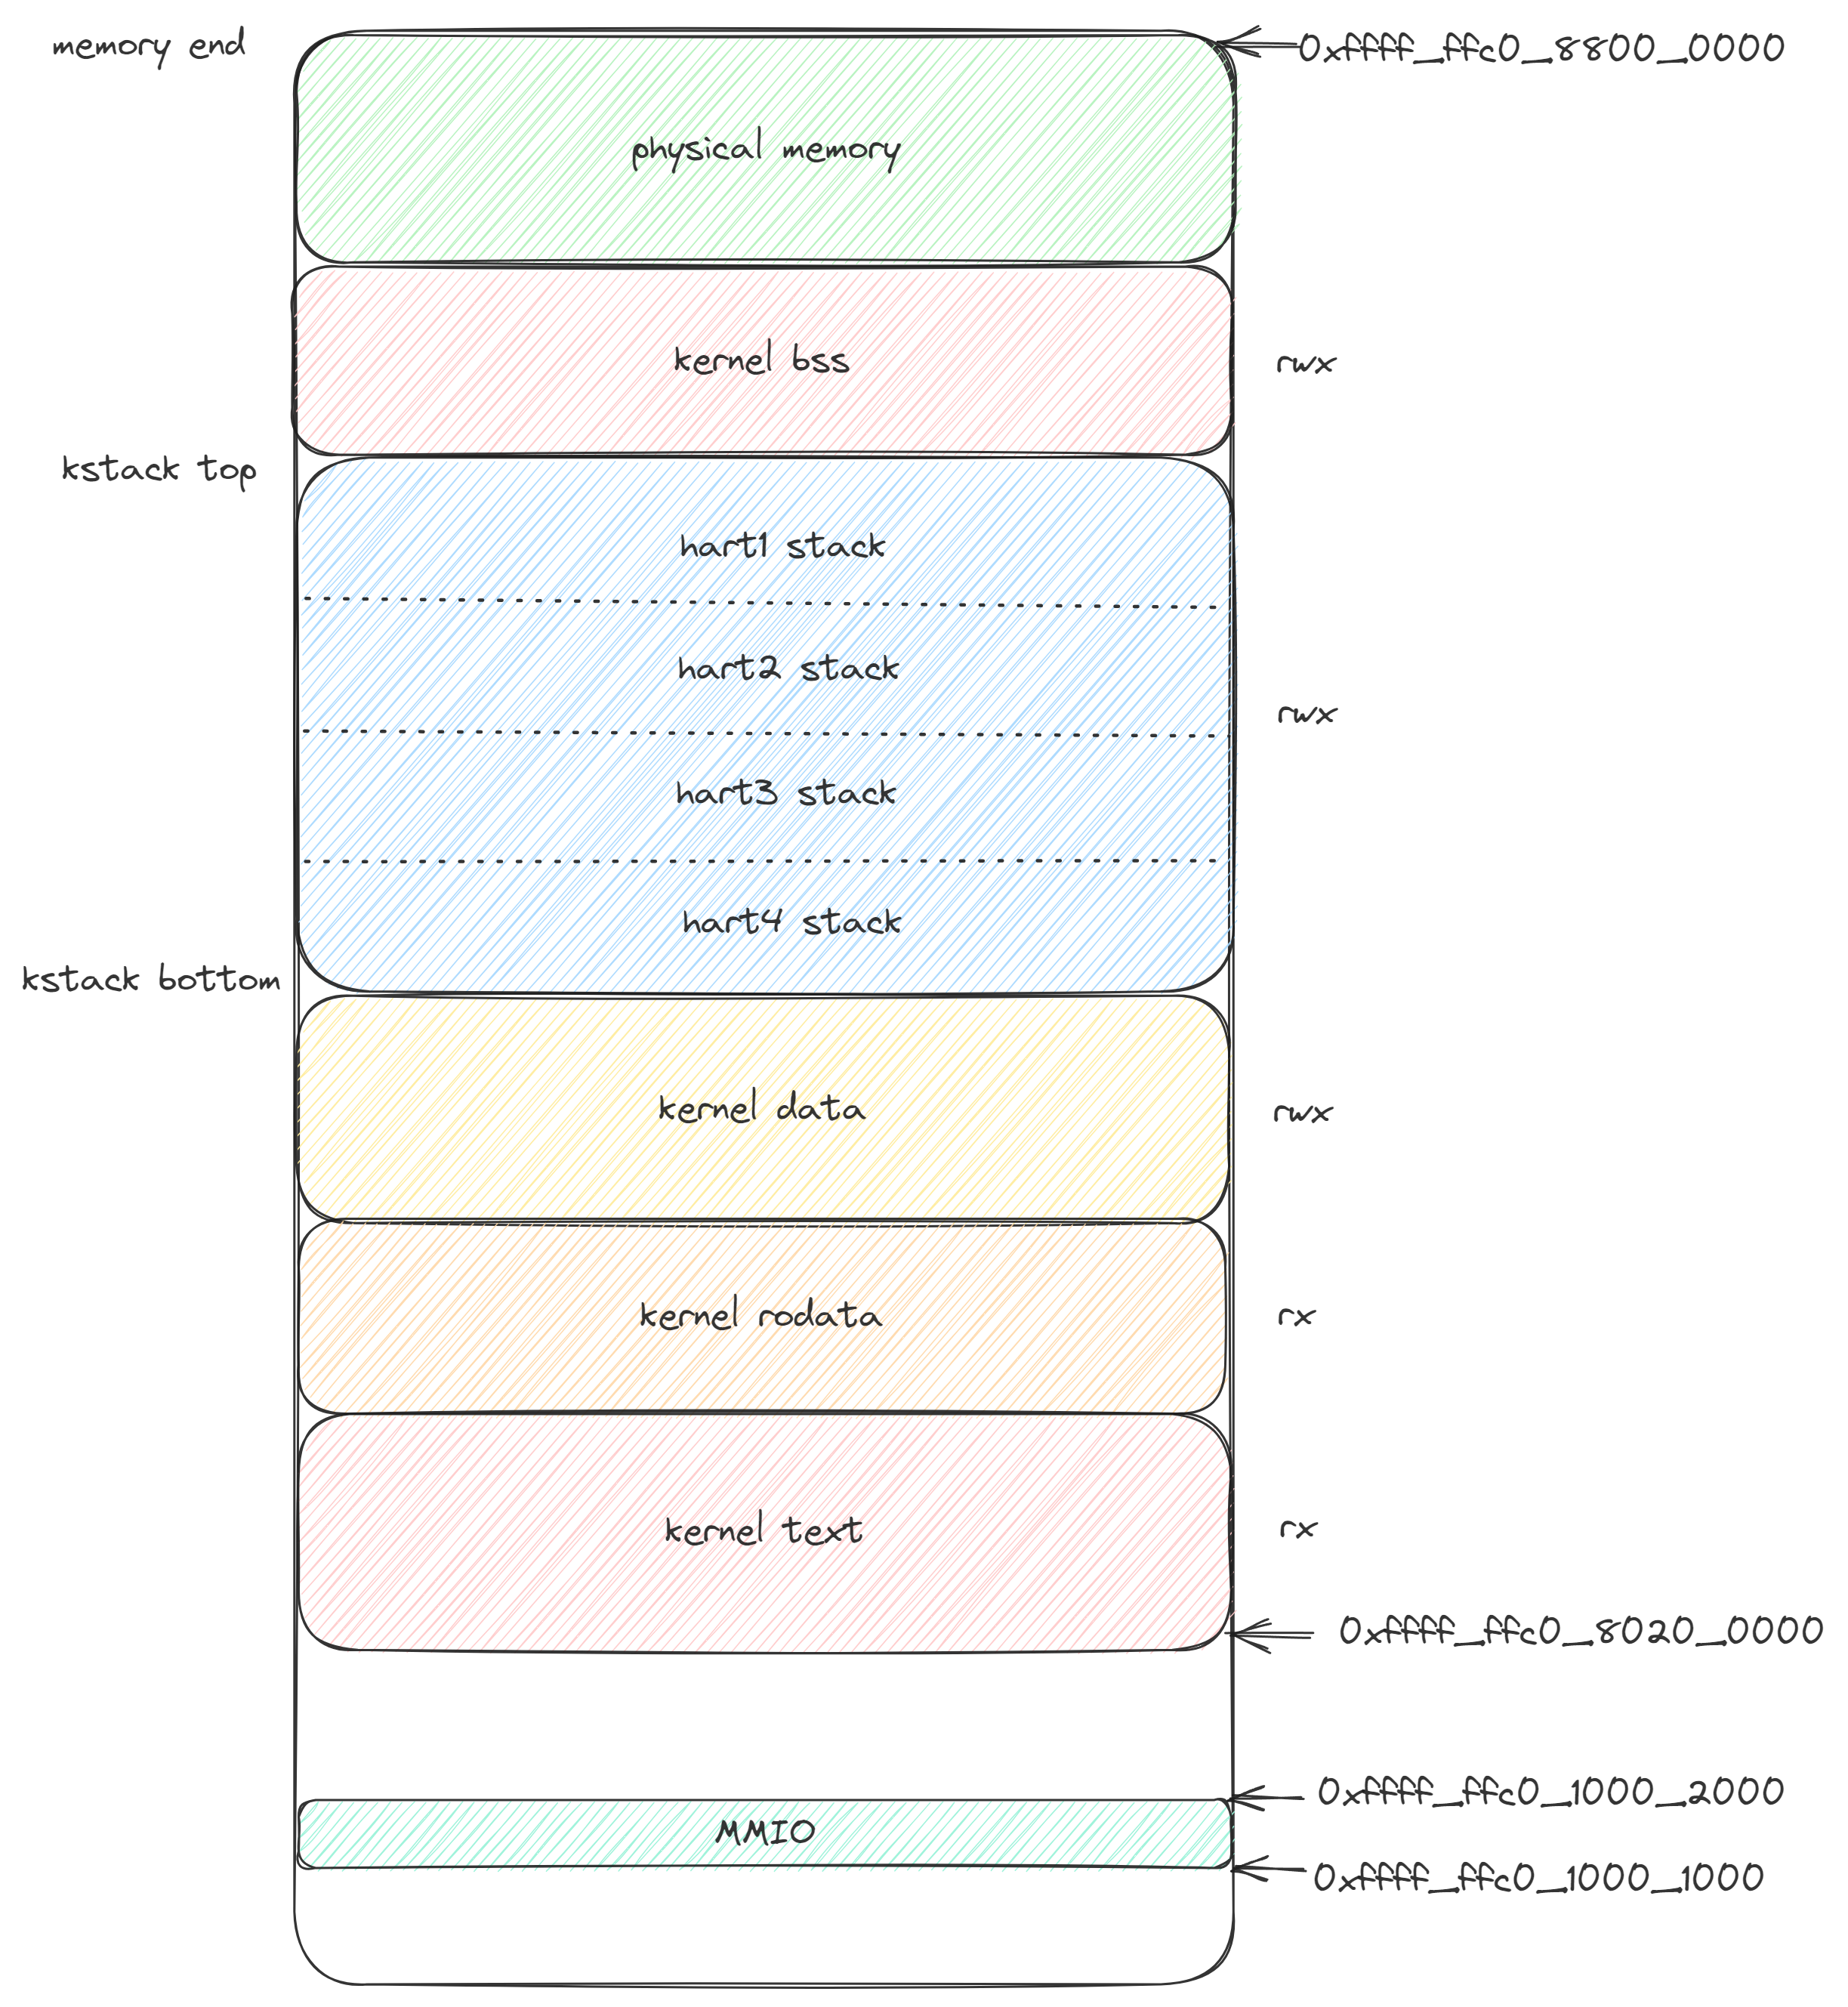
\includegraphics[width=.8\linewidth]{figure/kernel_mem.png}
    \caption{内核地址空间}
    \label{pic:kernel_mem}
\end{figure}

\paragraph{进入内核}~{}

那么如何在启动的时候快速映射到高位呢?我们难道要用汇编手写一个SV39三级页表?其实没必要,在RISC-V SV39里,MMU的翻译逻辑是逐级查找,一旦遇到页表项包含了V位,便停止查找,并不需要查满三层,这意味着我们可以直接映射一个巨页(即只用一级页表),手写一个根页表并不是一件非常复杂的事情,我们只需要将0x8000\_0000和0xffff\_ffc0\_8000\_0000这两个巨页添加到页表项即可,具体逻辑如下所示:
\begin{tcolorbox}[title=\textbf{os/src/entry.S}]
\begin{minted}[baselinestretch=1, fontsize=\small]{gas}
boot_pagetable:
    # we need 2 pte here
    # 0x0000_0000_8000_0000 -> 0x0000_0000_8000_0000
    # 0xffff_fc00_8000_0000 -> 0x0000_0000_8000_0000
    .quad 0
    .quad 0
    .quad (0x80000 << 10) | 0xcf # VRWXAD
    .zero 8 * 255
    .quad (0x80000 << 10) | 0xcf # VRWXAD
    .zero 8 * 253
\end{minted}
\end{tcolorbox}

另外,我们将内核的栈段划分为多段作为每个核心的内核栈,在进入内核的时候根据sbi传入的核心id计算出对应核心的内核栈的范围,并将其值赋给sp指针即可。

\paragraph{用户地址空间}~{}

用户地址空间见下\cref{pic:user_mem}所示,我们将文件映射及匿名映射的内存地址放置到用户地址空间的最高位,将堆段放置到栈段之上,其他的段都是在解析程序elf文件时映射的。

\begin{figure}[hbt]
    \centering
    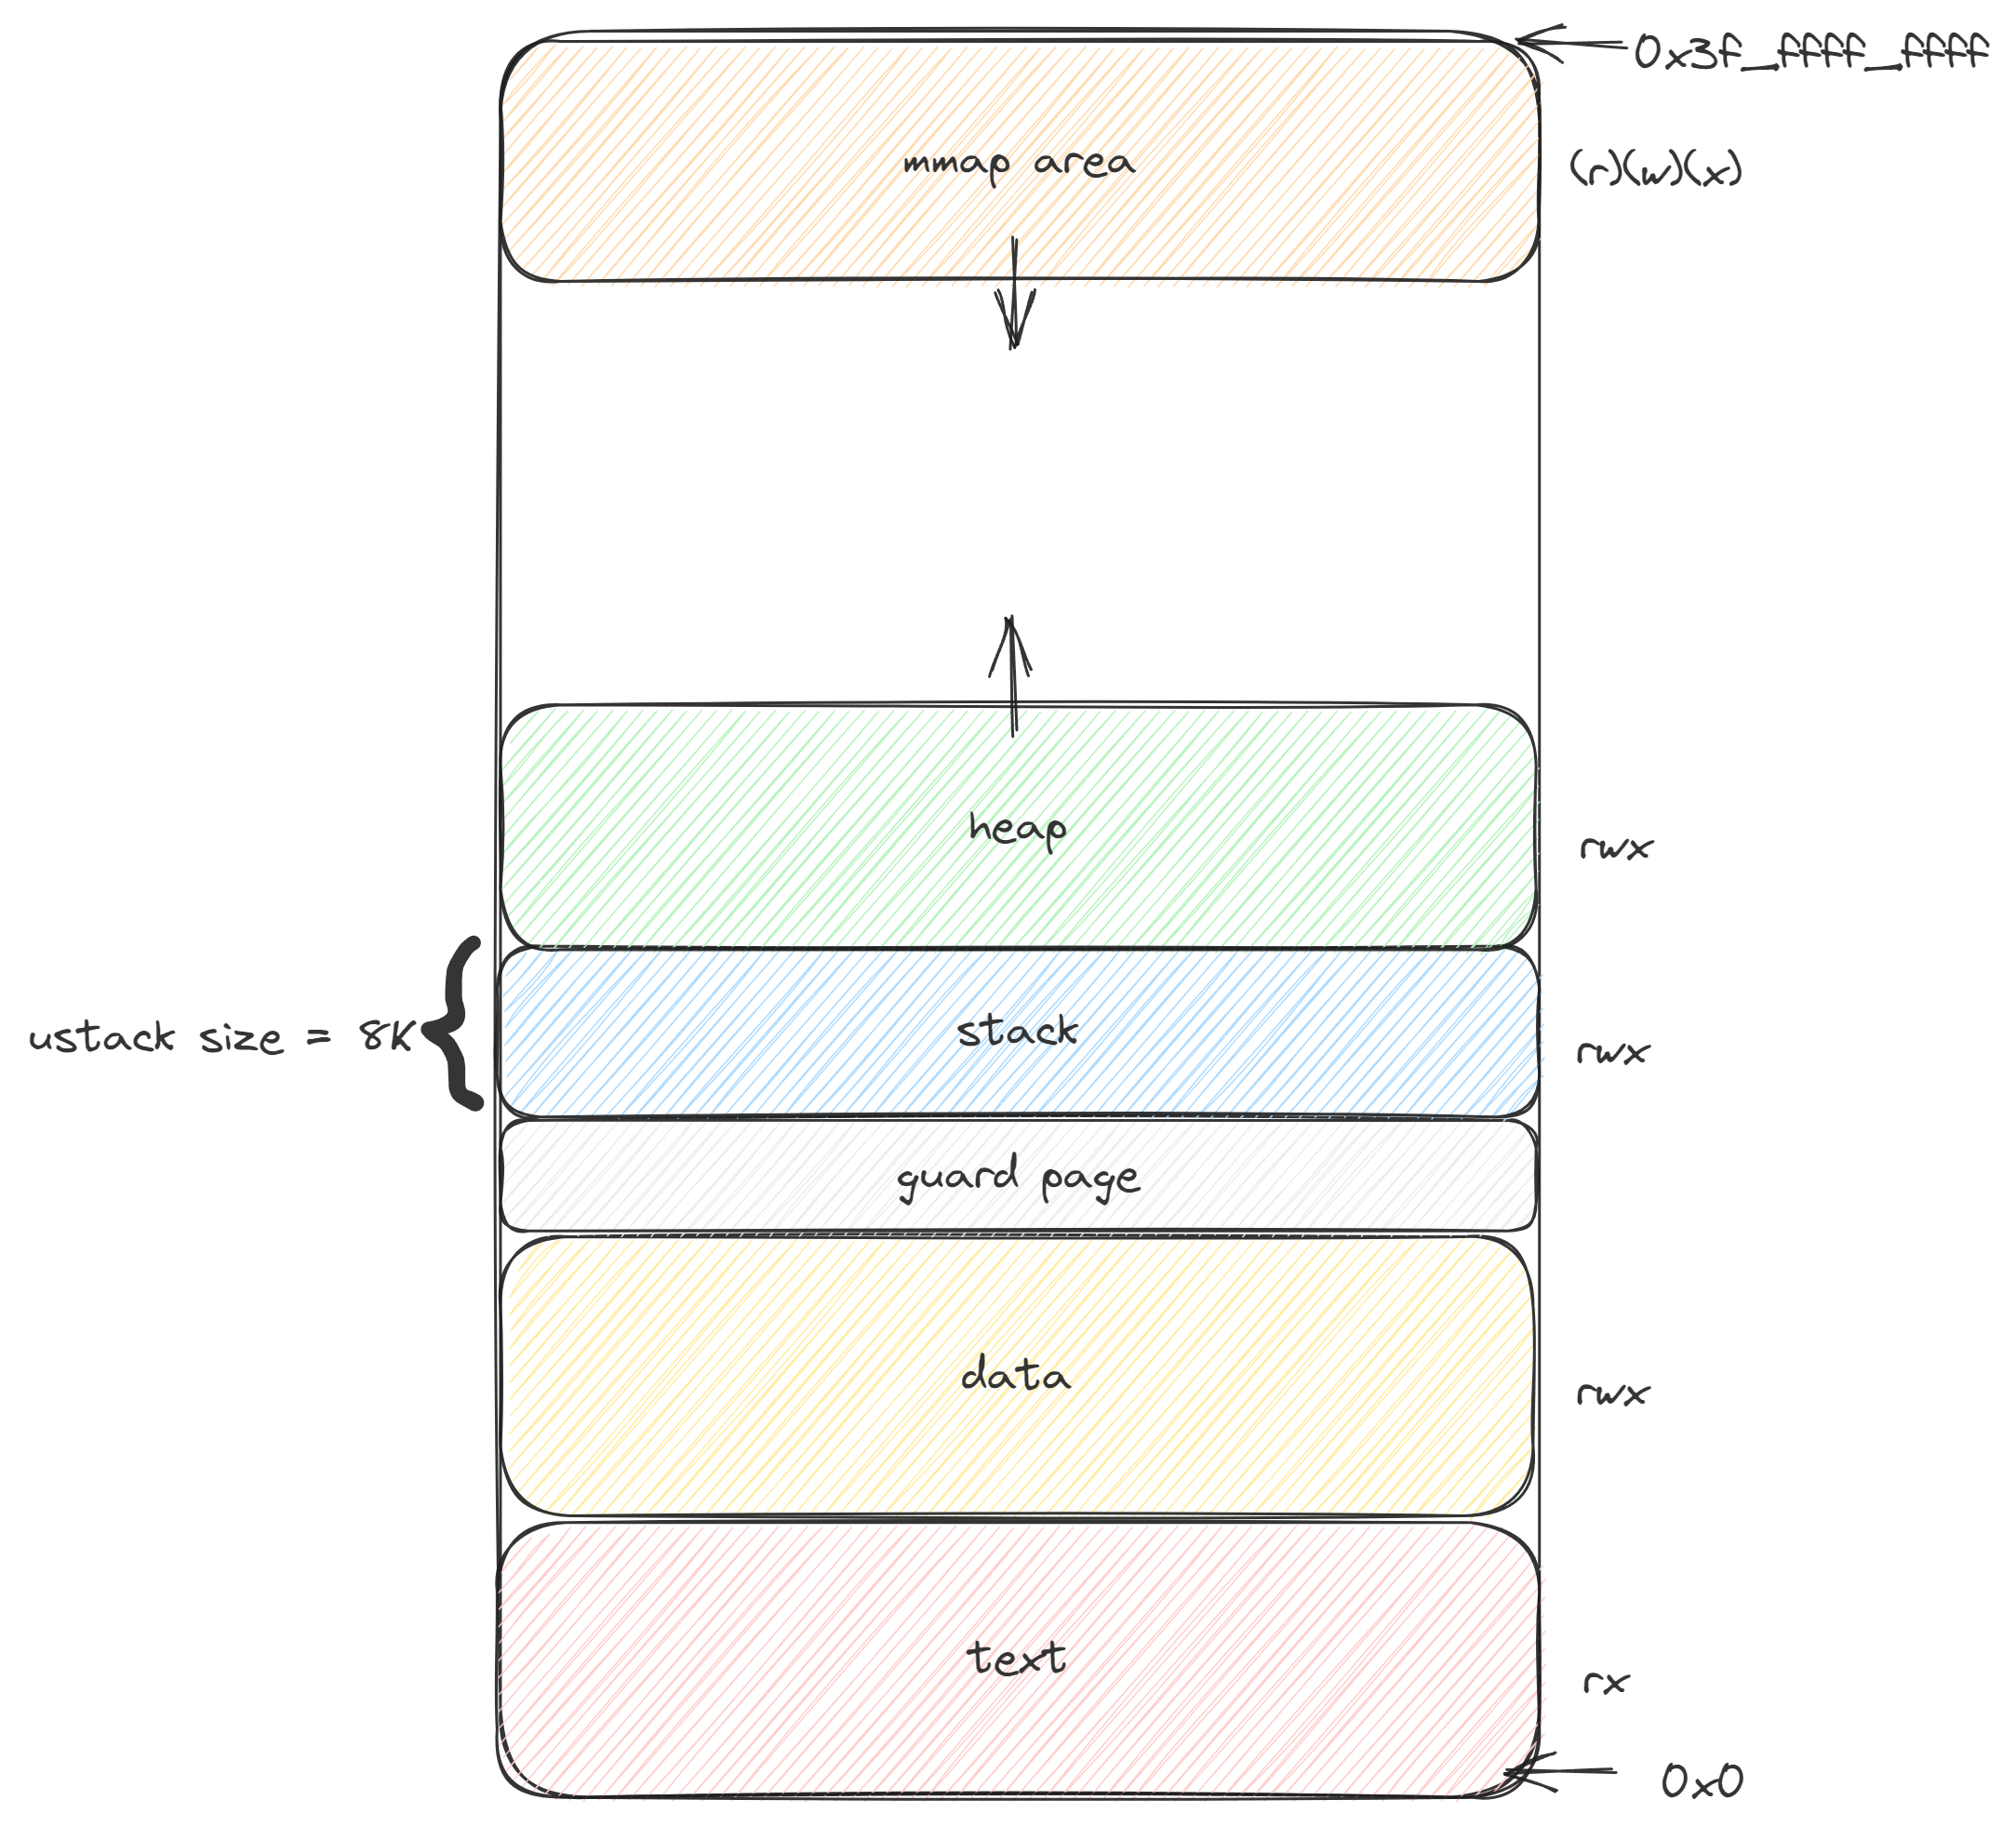
\includegraphics[width=.8\linewidth]{figure/user_mem.png}
    \caption{用户地址空间}
    \label{pic:user_mem}
\end{figure}

\subsubsection{内存映射}

\paragraph{内核空间内存映射}~{}

对于内核空间来说,所有的段都是直接映射,这里的直接映射指物理页地址加上一个偏移量(即0xffff\_ffc0),包括物理页帧,因此在将物理页帧分配给用户时需要将地址减去偏移量才能得到真正的物理地址。

\paragraph{用户空间内存映射}~{}

对于用户空间来说,所有的段都是物理页帧随机映射,我们在内核中维护一个物理页帧分配器用以管理所有的物理页帧,对于每个物理页帧,我们采用了Rust中的原子引用计数Arc来维护,当物理页帧的引用计数为0时自动释放,我们通过覆盖物理页帧的析构函数来实现将空闲物理页帧回收至物理页帧分配器,这是一种RAII的思想,广泛运用在我们的内核中,同时Arc也大大简化了后面我们实现写时复制的步骤。

\subsubsection{内存管理相关数据结构}
\begin{figure}[hbt]
    \centering
    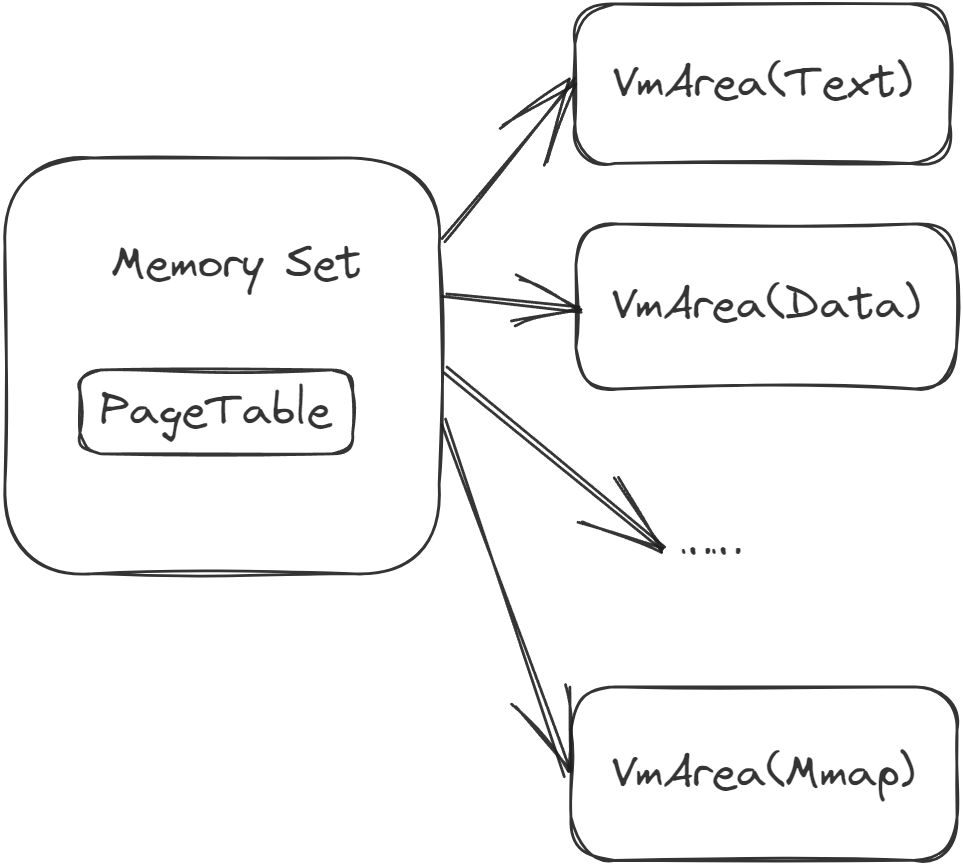
\includegraphics[width=.7\linewidth]{figure/mem_set.png}
    \caption{进程地址空间数据结构}
    \label{pic:mem_set}
\end{figure}

下面介绍内核中内存管理相关的重要数据结构。

\paragraph{MemorySet}~{}

\begin{tcolorbox}[title=\textbf{os/src/entry.S}]
\begin{minted}[baselinestretch=1, fontsize=\small]{rust}
/// memory set structure, controls virtual-memory space
pub struct MemorySet {
    /// we should ensure modifying page table exclusively(e.g. through process_inner's lock)
    /// TODO: optimization: decrease the lock granularity when handling page fault
    pub page_table: Arc<SyncUnsafeCell<PageTable>>,
    /// start vpn -> vm_area
    areas: BTreeMap<VirtPageNum, VmArea>,
    /// heap range
    pub heap_range: Option<HeapRange>,
}
\end{minted}
\end{tcolorbox}
如上所示,每个进程会有一个MemorySet成员表示其地址空间,该结构体包含一个页表,以及通过B树维护对各个内存段的索引,便于根据给定的虚拟地址快速查找、删除或修改其对应的内存段。

\paragraph{VmArea}~{}

\begin{tcolorbox}[title=\textbf{os/src/entry.S}]
\begin{minted}[baselinestretch=1, fontsize=\small]{rust}
/// map area structure, controls a contiguous piece of virtual memory
pub struct VmArea {
    /// Vpn range
    pub vpn_range: VPNRange,
    /// We don't need to use lock because we've locked the process
    /// inner every time we handle page fault
    pub data_frames: UnsafeCell<FrameManager>,
    /// Map type
    pub map_type: MapType,
    /// Map permission
    pub map_perm: MapPermission,
    /// Mmap flags
    pub mmap_flags: Option<MmapFlags>,
    /// Page fault handler that is invoked when page fault
    pub handler: Option<Box<dyn PageFaultHandler>>,
    /// Backup file(only used for mmap)
    pub backup_file: Option<BackupFile>,
}
\end{minted}
\end{tcolorbox}
如上所示,VmArea即代表某个内存段,各个成员的作用如注释所述,值得注意的是,VmArea有一个handler成员,当发生页错误时,我们可以根据发生页错误的地址查找出相应的VmArea,然后再调用其handler成员处理这个页错误,从而让页错误的维护工作变得统一且具有可扩展性。

\subsubsection{懒分配与写时复制}

为了提高性能,我们应当尽可能地减少拷贝和申请内存的次数,目前Titanix里采用了懒分配和写时复制的技术来减少开销。

\paragraph{懒分配}~{}

目前Titanix里的懒分配主要有以下三个方面:
\begin{enumerate}
    \item 用户栈的懒分配:在进程构建出来的时候,我们给用户进程划分一个虚拟地址栈空间但不实际分配物理地址,当用户访问栈空间时再通过缺页中断分配物理页。
    \item 用户堆的懒分配:类似与用户栈的懒分配,当用户调用brk系统调用增长进程空间时,我们只增长虚拟地址空间而不实际分配物理内存,当用户真正读写该堆空间时再通过缺页中断进行物理页分配。
    \item mmap内存段的懒读取:当用户进行mmap系统调用时,我们记录下对应的文件指针以及映射的偏移量范围但不进行实际读取,当用户真正读写到该内存段时再通过缺页中断读取相应文件的相应位置的内容。
\end{enumerate}

\paragraph{写时复制}~{}

当进行fork系统调用构造出新的进程时,我们不需要将父进程地址空间的全部内存拷贝一份,而是让子进程与父进程共享物理内存页,这样做的开销就只有修改页表了。注意到RISC-V中页表项的标志位中留了一个保留位,我们可以将其设置为COW位,在fork的时候需要将具有写权限的内存段的写标志位去掉,同时添上COW位。值得注意的是,在copy-on-write的时候我们还需要注意某个内存段是否是懒分配的内存段,若是,我们便不需要共享物理页,直接新增一个虚拟地址内存段即可。

另外,前文提到我们对物理页帧使用Arc(原子引用计数)进行维护,在这里派上了用场,因为在COW的时候父子进程会同时持有对同一物理页面的所有权,对于一个物理页面,我们需要等到其引用计数为0的时候才可以将其回收进空闲物理页帧中,这里直接利用了Arc的特性。

\paragraph{页错误处理函数}~{}

懒分配和写时复制在后面还需要进行扩展,如elf文件懒加载等,而这项技术的关键在于通过缺页中断进行真正的分配或者加载,因此我们需要设计一个可扩展的统一的页错误处理方式以便于后期的维护与扩展。通过参考Linux,我们为每个内存段(VmArea)设置一个页错误处理函数,利用Rust里的动态分发实现多态,从而可以使用统一的接口来存储页错误处理函数,该trait如下所示:
\begin{tcolorbox}[title=\textbf{os/src/mm/memory\_set/page\_fault\_handler.rs}]
\begin{minted}[baselinestretch=1, fontsize=\small]{rust}
/// General page fault handler
pub trait PageFaultHandler: Send + Sync {
    /// Handle the specific virtual page fault
    fn handle_page_fault(
        &self,
        va: VirtAddr,
        vma: &VmArea,
        page_table: &mut PageTable,
    ) -> GeneralRet<()>;

    ///
    fn is_legal(&self, _scause: Scause) -> bool {
        todo!();
    }

    /// Used for cloning in `fork`
    fn box_clone(&self) -> Box<dyn PageFaultHandler>;
}
\end{minted} 
\end{tcolorbox}

\subsubsection{用户地址检查}

在Titanix中,用户和内核共享地址空间,因此在访问用户态的内存时不需要同Xv6那样通过软件查询页表,而可以直接解引用访问。但直接解引用会带来一个问题,如果用户态传入的地址是一个不合法的地址,那在内核态直接解引用就会导致内核崩溃,因此对于用户态传入的地址,我们需要谨慎判断。我们采用这样一个方案,首先实现一个内核态异常的处理函数,当想要读写某个用户地址段时,先将修改中断向量的值为以下汇编函数的地址:
\begin{tcolorbox}[title=\textbf{os/src/mm/memory\_set/page\_fault\_handler.rs}]
\begin{minted}[baselinestretch=1, fontsize=\small]{rust}
// if pagefault occurs, return: (a0, a1) <- (1, scause).
    .align 6
__try_access_user_error_trap:
    csrw sepc, ra   # ra -> __try_x_user_u8's return addr
    li a0, 1
    csrr a1, scause
    sret
\end{minted} 
\end{tcolorbox}
以上函数即为

\subsubsection{多核启动}


\subsubsection{页缓存}